
\documentclass{article}

\usepackage{hyperref}
\usepackage{listings}
\usepackage{graphicx}
\newcommand{\email}[1]{\href{mailto:#1}{#1}}

\newcommand{\sql}[1]{\lstinputlisting[language=sql]{sql/#1.sql}}


\title{
  Database Design Project\\
  IT 30
}
\author{
  Samuel Grahn, \email{samuel.grahn@outlook.com}\\
  Olof Bergenholtz, \email{obergenholtz@gmail.com}\\
  Masood Ahmed Rafay, \email{Rafayqureshi2010@gmail.com}\\
  Ali Kamran, \email{alkmrn1@gmail.com}\\
}

\begin{document}

\maketitle
\newpage
\section*{ER-diagram}
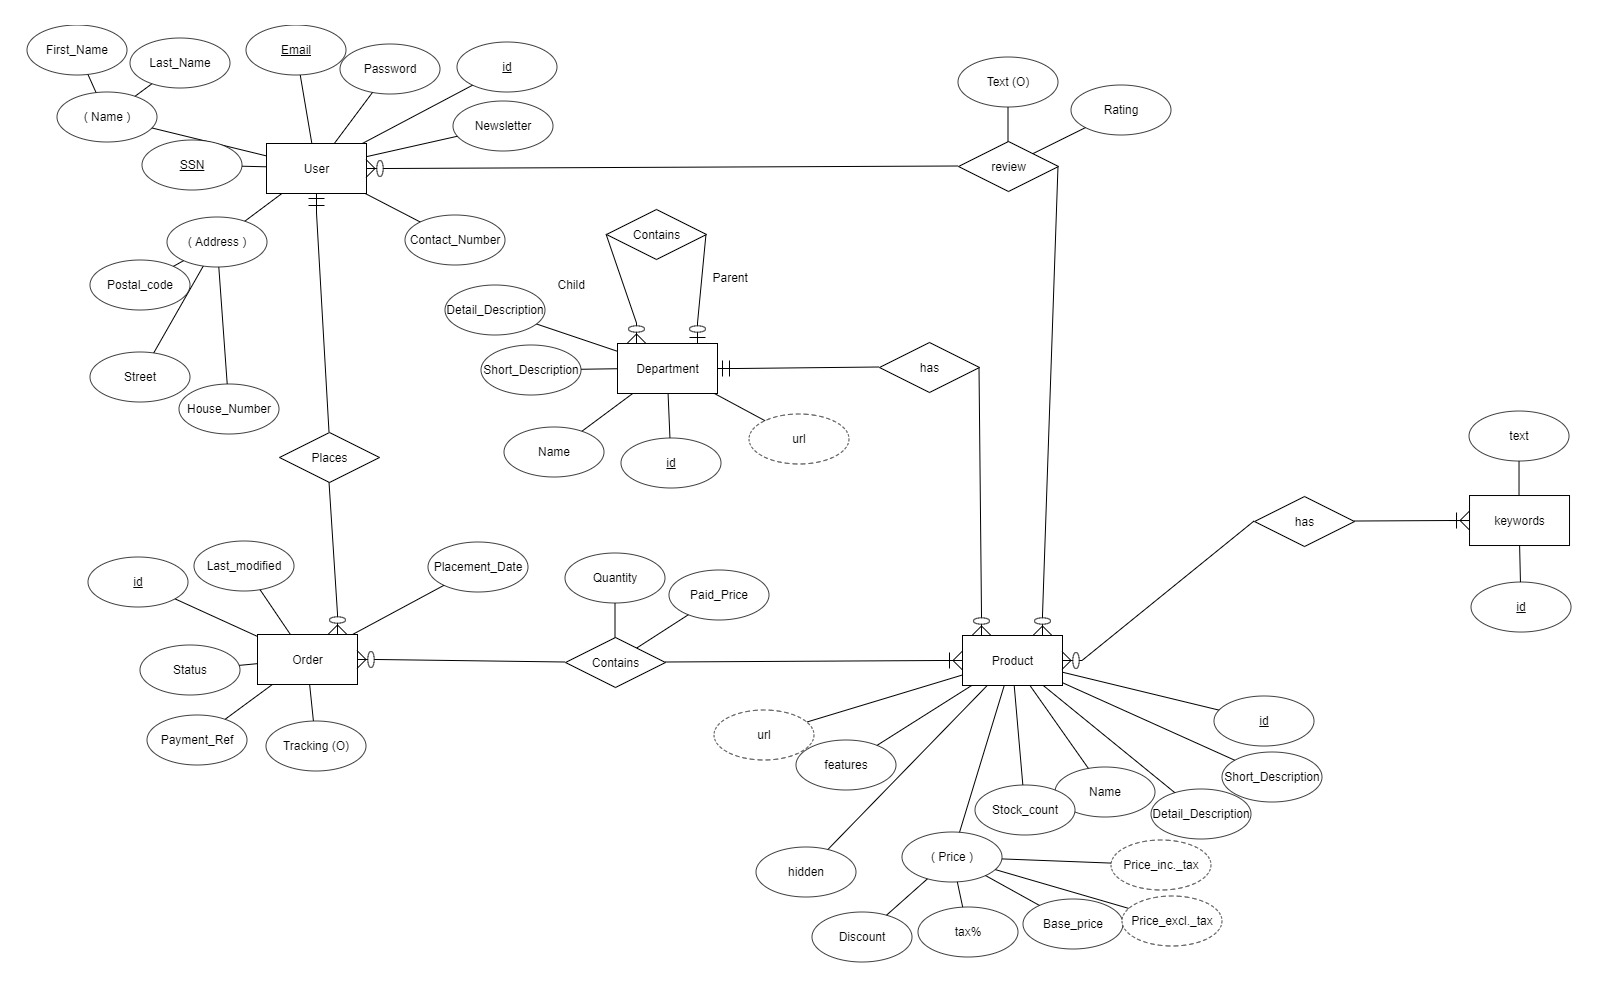
\includegraphics[height=\linewidth,angle=90]{er.png}

\section*{Generating the Database}
\sql{table_generation}

\section*{Task 4 Queries}
Welcome Text
\sql{welcome}
List of top-level departments
\sql{topleveldpt}
List of featured products
\sql{featured_products}
List all keyword-related producs to a product
\sql{similar_products}
List all products in a given department
\sql{dept_products}
List all products on sale sorted by discount percentage
\sql{sale}

\section*{Task 5 Indices}
To improve the query for featured products, we create an index using\\
\sql{indices}

Running
\sql{explain}
before and after creating this index yields\\
\begin{tabular}{ | c c c c c c c c c c | }
  \hline
  id & select\_type & table & type & possible\_keys & key & key\_len & ref & rows & extra\\
  \hline
  1 & SIMPLE & products & ALL & NULL & NULL & NULL & NULL & 11 & Using where\\
  1 & SIMPLE & products & ref & featured\_idx & featured\_idx & 2 & const & 5 & NULL\\
  \hline
\end{tabular}

\end{document}
